\subsection{Alignment Tuning}
\label{sec-alignment}

This part first presents the background of alignment with its definition and criteria, then focuses on the collection of human feedback data for aligning LLMs, and finally discusses the key technique of reinforcement learning from human feedback (RLHF) for alignment tuning. 

\subsubsection{Background and Criteria for Alignment}
\label{sec-alignment-background}
\paratitle{Background.} LLMs have shown remarkable capabilities in a wide range of NLP tasks~\cite{Brown-NeurIPS-2020-Language,Chowdhery-arxiv-2022-PaLM,Wei-ICLR-2022-Finetuned,Zhang-arxiv-2022-OPT}. However, these models may sometimes exhibit  unintended behaviors, \eg  fabricating false information, pursuing inaccurate objectives, and producing harmful, misleading, and biased expressions~\cite{Ouyang-arxiv-2022-Training,Kenton-arxiv-2021-Alignment}. For LLMs, the language modeling objective pre-trains the model parameters by word prediction while lacking the consideration of human values or preferences.    
{To avert these unexpected behaviors, human alignment has been proposed to make LLMs act in line with human expectations}~\cite{Ouyang-arxiv-2022-Training,Ziegler-arxiv-2019-Fine-Tuning}.  
However, unlike the original pre-training  and adaptation tuning (\eg instruction tuning), such an alignment requires considering very different criteria  (\eg helpfulness, honesty, and harmlessness).  It has been shown that alignment might harm the general abilities of LLMs to some extent, which is called \emph{alignment tax} in related literature~\cite{Askell-arxiv-2021-A}.  
 
\paratitle{Alignment Criteria.} 
{Recently, there is increasing attention on developing multifarious criteria to regulate the behaviors of LLMs. 
Here, we take three representative alignment criteria (\ie helpful, honest, and harmless) as examples for discussion, which have been widely adopted  in existing literature~\cite{Askell-arxiv-2021-A,Ouyang-arxiv-2022-Training}. 
}
In addition, there are  other alignment criteria for LLMs from different  perspectives including behavior, intent, incentive, and inner aspects~\cite{Kenton-arxiv-2021-Alignment}, which are essentially similar (or at least with similar  alignment techniques) to the above three criteria. 
It is also feasible to modify the three criteria according to specific needs, \eg substituting honesty with correctness~\cite{Glaese-arxiv-2022-Improving}.   
Next, we give brief explanations about the three representative alignment criteria:

$\bullet$ \emph{Helpfulness.} To be helpful, the LLM should demonstrate a clear attempt to assist users in solving their tasks or answering questions in a concise and efficient manner as possible. At a higher level, when further clarification is needed, the LLM should demonstrate the capability of eliciting  additional relevant information through pertinent inquiries and exhibit suitable levels of sensitivity, perceptiveness, and prudence~\cite{Askell-arxiv-2021-A}. Realizing the alignment of helpful behavior is challenging for LLMs since it is difficult to precisely define and measure the intention of users~\cite{Kenton-arxiv-2021-Alignment}.

$\bullet$ \emph{Honesty.} At a basic level, a LLM aligned to be honest should present accurate content to users instead of fabricating information. Additionally, it is crucial for the LLM to convey appropriate degrees of uncertainty in its output, in order to avoid any form of deception or misrepresentation of information. This requires the model to know about its capabilities and levels of knowledge (\eg ``know unknowns''). According to the discussion in \cite{Askell-arxiv-2021-A}, honesty is a more objective criterion compared to helpfulness and harmlessness, hence honesty alignment could potentially be developed with less reliance on human efforts. 

$\bullet$ \emph{Harmlessness.} To be harmless, it requires that the language produced by the model should not be offensive or discriminatory. To the best of its abilities, the model should be capable of detecting covert endeavors aimed at soliciting requests for malicious purposes. Ideally, when the model was  induced to conduct a dangerous action (\eg committing a crime), the LLM should politely refuse. Nonetheless, 
\emph{what behaviors} are deemed harmful and \emph{to what extent} vary amongst individuals or  societies~\cite{Askell-arxiv-2021-A} highly  depend on who is using the LLM, the type of the posed question, and the context (\eg time) at which the LLM is being used.

As we can see, these criteria are quite subjective, and are developed based on human cognition. 
Thus, it is difficult to directly formulate them as optimization objectives for LLMs. 
{In existing work, there are many ways to fulfill these criteria when aligning LLMs. 
A promising technique is \emph{red teaming}~\cite{Perez-EMNLP-2022-Red}, which involves using manual or automated means to probe LLMs in an adversarial way to generate harmful outputs and then updates LLMs to prevent such outputs.

\subsubsection{Collecting Human Feedback}\label{sec-human-feedback}
During the pre-training stage, LLMs are trained using the language modeling objective on a large-scale corpus. However, it cannot take into account the subjective and qualitative evaluations of LLM outputs by humans (called \emph{human feedback} in this survey).
High-quality human feedback is extremely important for aligning LLMs with human preferences and values.
In this part, we discuss how to select a team of human labelers for  feedback data collection.  

\paratitle{Human Labeler Selection.}  
In existing work, the dominant method for generating human feedback data is human annotation~\cite{Ziegler-arxiv-2019-Fine-Tuning,Ouyang-arxiv-2022-Training,Glaese-arxiv-2022-Improving}. This highlights the critical role of selecting appropriate human labelers.
To provide high-quality feedback, human labelers are supposed to have a qualified level of education and excellent proficiency in English. For example, Sparrow~\cite{Glaese-arxiv-2022-Improving} requires human labelers to be UK-based native English speakers who have obtained at least an undergraduate-level educational qualification.
Even then, several studies~\cite{Ziegler-arxiv-2019-Fine-Tuning} have found that there still exists a mismatch between the intentions of researchers and human labelers, which may lead to low-quality human feedback and cause LLMs to produce unexpected output. 
To address this issue, %
InstructGPT~\cite{Ouyang-arxiv-2022-Training} further conducts a screening process to filter labelers by assessing the agreement between human labelers and researchers. Specifically, researchers first label a small amount of data and then measure the agreement between themselves and human labelers. The labelers with the highest agreement will be selected to proceed with the subsequent annotation work. 
In some other work~\cite{Menick-arxiv-2022-teaching},  ``super raters'' are used to ensure the high quality of human feedback. Researchers evaluate the performance of human labelers and select a group of well-performing human labelers (\eg high agreement) as super raters. The super raters will be given priority to collaborate with the researchers in the subsequent study. 
When human labelers annotate the output of LLMs, it is helpful to specify detailed instructions and provide instant guidance for human labelers, which can further regulate the annotation of labelers. 



\paratitle{Human Feedback Collection.}  In existing work, there are mainly three kinds of approaches to collecting  feedback and preference data from human labelers.

$\bullet$ \emph{Ranking-based approach.} In early work~\cite{Ziegler-arxiv-2019-Fine-Tuning}, human labelers often evaluate model-generated outputs in a coarse-grained manner (\ie only selecting the best) without taking into account more fine-grained alignment criteria. Nonetheless, different labelers may hold diverse opinions on the selection of the best candidate output, and this method disregards the unselected samples, which may lead to inaccurate or incomplete human feedback.
To address this issue, subsequent studies~\cite{Glaese-arxiv-2022-Improving} introduce {the Elo rating system} to derive the preference ranking by comparing candidate outputs. 
{The ranking of outputs serves as the training signal that guides the model to prefer certain outputs over others, thus inducing outputs that are more reliable and safer.} 

$\bullet$ \emph{Question-based approach.}
Further, human labelers can provide more detailed feedback by answering certain questions designed by researchers~\cite{Nakano-arxiv-2021-WebGPT}, covering the alignment criteria as well as additional constraints for LLMs. Specially, in WebGPT~\cite{Nakano-arxiv-2021-WebGPT}, to assist the model in  filtering and utilizing relevant information from retrieved documents, human labelers are required to answer questions with multiple options about whether the retrieved documents are useful for answering the given input. 

$\bullet$ \emph{Rule-based approach.}
Many studies also develop rule-based methods to provide more detailed human feedback.
As a typical case, Sparrow~\cite{Glaese-arxiv-2022-Improving} not only selects the response that labelers consider the best but also uses a series of rules to test whether model-generated responses meet the alignment criteria of being helpful, correct, and harmless.  
In this way, two kinds of human feedback data can be obtained: (1) the response preference feedback is obtained by comparing the quality of model-generated output in pairs, and (2) the rule violation feedback is obtained by collecting the assessment from human labelers (\ie a score indicating to what extent the generated output has violated the rules). 
{Furthermore,  GPT-4~\cite{OpenAI-OpenAI-2023-GPT-4} utilizes a set of zero-shot classifiers (based on GPT-4 itself) as rule-based reward models, which can automatically determine whether the model-generated outputs violate a set of human-written rules.
}

In the following, we focus on a well-known technique, reinforcement learning from human feedback (RLHF), which has been widely  used in the recent powerful LLMs such as ChatGPT.} As discussed below, the alignment criteria introduced in %
{Section~\ref{sec-alignment-background}} can be fulfilled by learning from human feedback on the responses of LLMs to users' queries. 

\subsubsection{Reinforcement Learning from Human Feedback}\label{sub:RLHF}

\begin{figure}
    \centering
    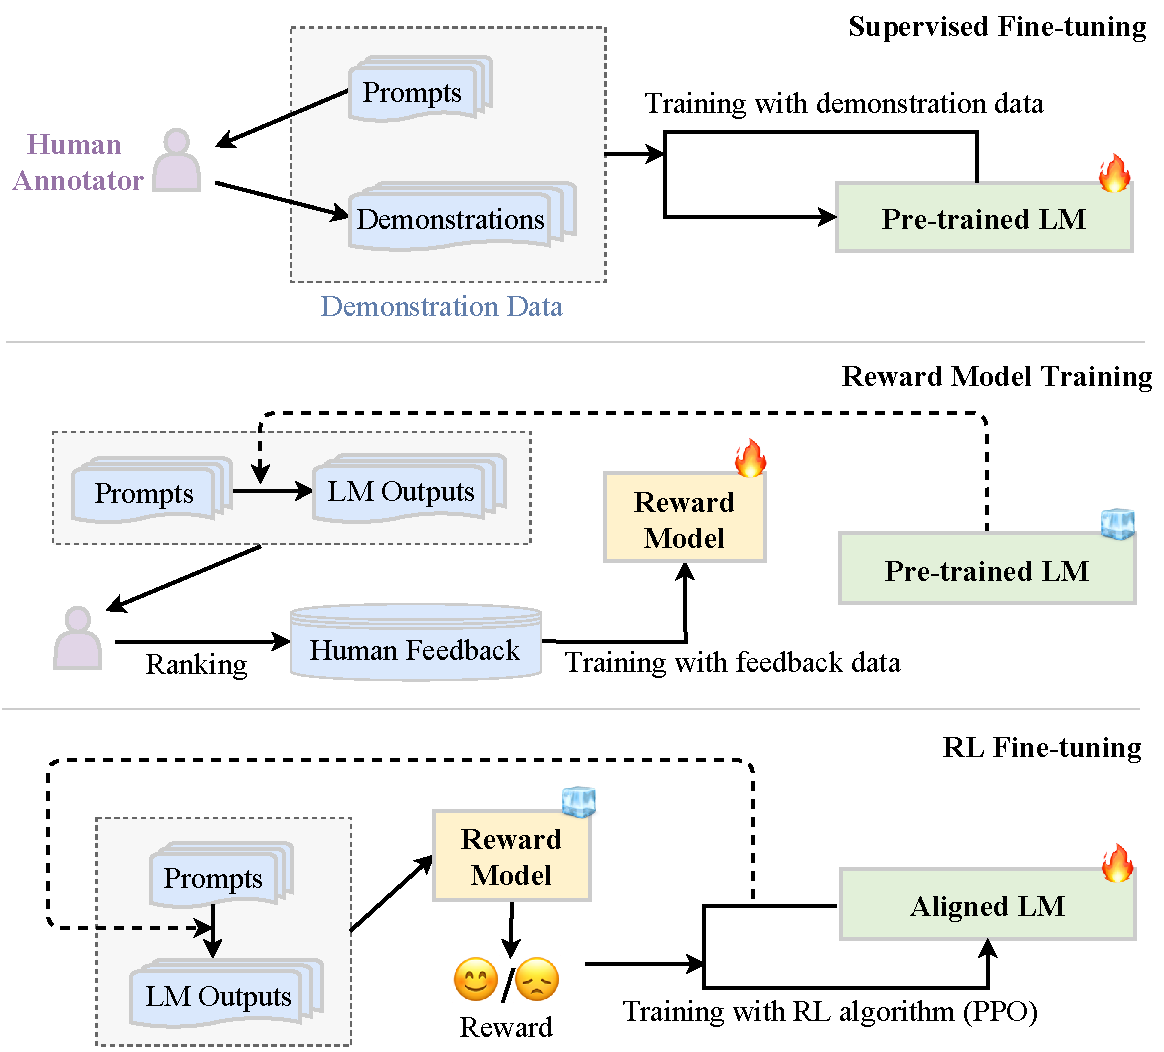
\includegraphics[width=0.5\textwidth]{images/RLHF.pdf}
    \caption{The workflow of the RLHF algorithm.}
    \label{fig:RLHF}
\end{figure}

To align LLMs with human values, reinforcement learning from human feedback (RLHF)~\cite{Christiano-NeurIPS-2017-Deep,Ziegler-arxiv-2019-Fine-Tuning} has been proposed to fine-tune LLMs with the collected human feedback data, which is useful to improve the alignment criteria (\eg helpfulness, honesty, and harmlessness).
RLHF employs reinforcement learning~(RL) algorithms~(\eg Proximal Policy Optimization~(PPO)~\cite{schulman-arxiv-2017-proximal}) to  adapt LLMs to human feedback by learning a reward model. Such an approach incorporates humans in the training loop for developing well-aligned LLMs, as exemplified by InstructGPT~\cite{Ouyang-arxiv-2022-Training}. 

\begin{figure*}[!t]
    \centering
    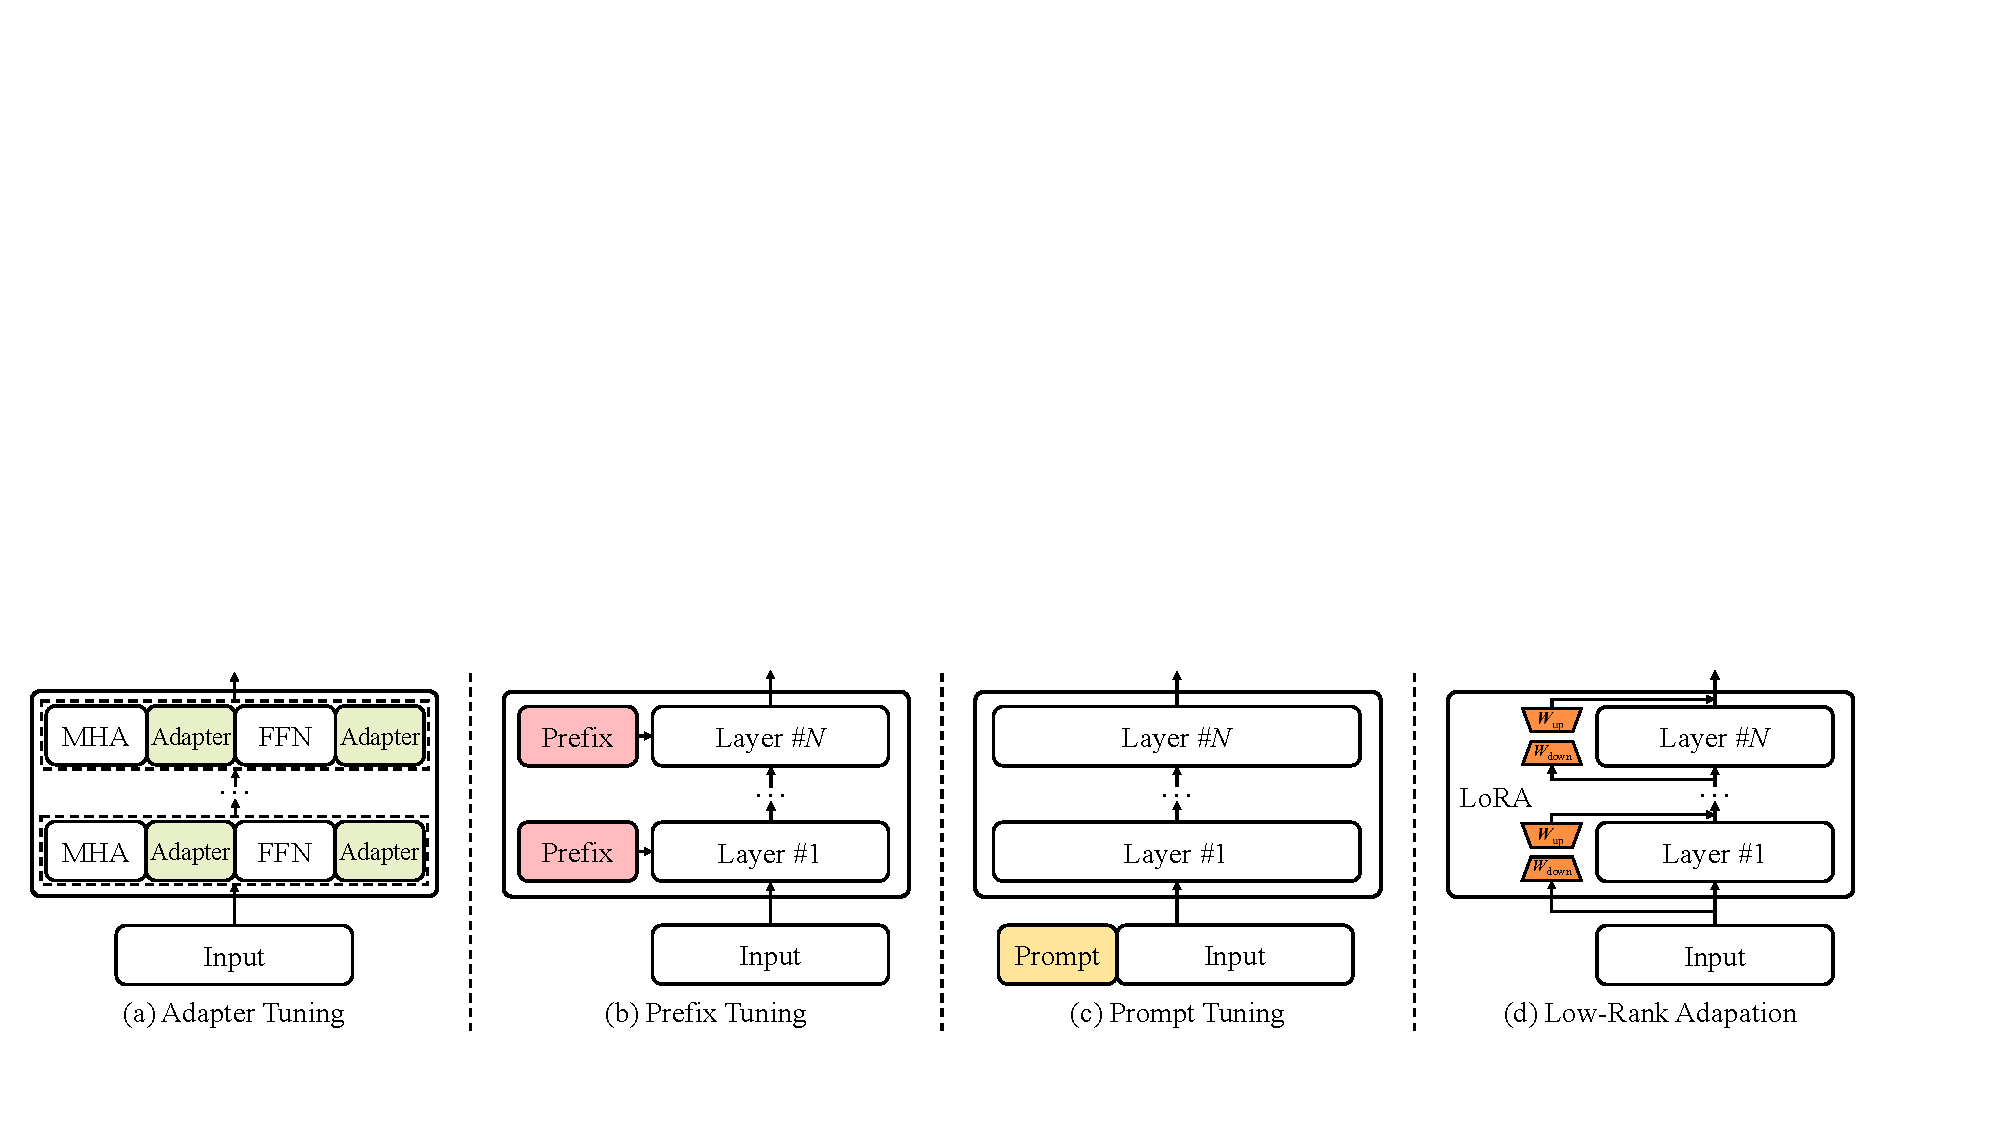
\includegraphics[width=1\textwidth]{images/Efficient-Tuning.pdf}
    \caption{An illustration of four different parameter-efficient fine-tuning methods. MHA and FFN denote the multi-head attention and feed-forward networks in the Transformer layer, respectively.}
    \label{fig:efficient-tuning}
\end{figure*}

\paratitle{RLHF System.}
The RLHF system mainly comprises three key components: a pre-trained LM to be aligned, a reward model learning from human feedback, and a RL algorithm training the LM.  
Specifically, the \textit{pre-trained LM} is typically a generative model that is  initialized with existing pre-trained LM parameters. For example, OpenAI uses 175B GPT-3 for its first popular RLHF model, InstructGPT~\cite{Ouyang-arxiv-2022-Training}, and DeepMind uses the 280 billion parameter model Gopher~\cite{Rae-arxiv-2021-Scaling} for {its GopherCite model~\cite{Menick-arxiv-2022-teaching}. } %
Further, the \textit{reward model~(RM)} provides (learned) guidance signals that reflect human preferences for the text generated by the LM, usually in the form of a scalar value. The reward model can take on two forms: a fine-tuned LM or a LM trained de novo using human preference data.
{Existing work typically employs reward models having  a  parameter scale different from that of the aligned LM~\cite{Menick-arxiv-2022-teaching,Ouyang-arxiv-2022-Training}.} For example, OpenAI uses 6B GPT-3 and DeepMind uses 7B Gopher as the reward model, respectively.
Finally, to optimize the pre-trained LM using the signal from the reward model, a specific \textit{RL algorithm} is designed for large-scale model tuning. Specifically, Proximal Policy Optimization (PPO)~\cite{schulman-arxiv-2017-proximal} is a widely used RL algorithm for alignment in existing work~\cite{Ouyang-arxiv-2022-Training,Menick-arxiv-2022-teaching,Glaese-arxiv-2022-Improving}. 

\paratitle{Key Steps for RLHF.} Figure~\ref{fig:RLHF} illustrates the overall three-step process of RLHF~\cite{Ouyang-arxiv-2022-Training} as introduced below. 

$\bullet$ \textit{Supervised fine-tuning.} To make the LM initially perform desired behaviors, it  usually needs to collect a supervised dataset containing input prompts (instruction) and desired outputs for fine-tuning the LM. These prompts and outputs can be written by human labelers for some specific  tasks while ensuring the diversity of tasks.  
{For example, InstructGPT~\cite{Ouyang-arxiv-2022-Training} asks human labelers to compose prompts (\eg ``\emph{List five ideas for how to regain enthusiasm for my career}'') and desired outputs for several generative tasks such as open QA, brainstorming, chatting, and rewriting. }
Note that the first step is optional in specific settings or scenarios. 

$\bullet$ \textit{Reward model training.} The second step is to train the RM using human feedback data. Specifically, we employ the LM to generate a certain number of output texts using sampled prompts (from either the supervised dataset or the human-generated prompt) as input. We then invite human labelers to annotate the preference for these pairs. The annotation process can be conducted in multiple forms, and a common approach is to annotate by ranking the generated candidate texts, which can reduce  the inconsistency among annotators. Then,  the RM is trained to predict the human-preferred output. In InstructGPT, labelers rank model-generated outputs from best to worst, and the RM (\ie 6B GPT-3) is trained to predict the ranking. Note that, in recent work~\cite{Bai-arXiv-2022-Constitutional}, the annotation of preference on response pairs has been conducted by an AI agent (usually an aligned LLM) instead of humans, which is called ``\emph{reinforcement learning from AI feedback (RLAIF)}''. 
{LLMs trained with typical RLHF algorithms tend to generate harmless responses with less helpfulness, which is  called  \emph{evasion problem}~\cite{Bai-arXiv-2022-Constitutional}. To  guarantee both the harmlessness and helpfulness, RLAIF generates the AI feedback based on pre-set alignment principles in instructions~\cite{Bai-arXiv-2022-Constitutional,Lee-CoRR-2023-RLAIF}, which can also reduce  the efforts of human annotation.} 


$\bullet$ \textit{RL fine-tuning.} At this step, aligning (\ie fine-tuning) the LM is formalized as an RL problem. In this setting, the pre-trained LM acts as the policy that takes as input a prompt and returns an output text, the action space of it is the vocabulary, the state is the currently generated token sequence, and the reward is provided by the RM. To avoid eviating significantly from the initial (before tuning) LM, a penalty term is commonly incorporated into the reward function. 
For example, InstructGPT optimizes the LM against the RM using the PPO algorithm. 
For each input prompt, InstructGPT calculates the KL divergence between the generated results from the current LM and the initial LM as the penalty.
It is noted that the second and final steps can be iterated in multiple turns for better aligning LLMs. 
Due to the instability of the RL algorithm, recent work~\cite{Dong-RAFT-2023-arxiv} replaces the RL tuning with another supervised fine-tuning by reusing the best ranked samples with higher rewards.

\paratitle{Practical Strategies for RLHF.}
{Although RLHF is promising to effectively improve the alignment of LLMs with humans, it is practically challenging for researchers to successfully implement  it.
In this part, we focus on discussing several useful  strategies and tricks for improving the effectiveness and efficiency of RLHF. 
Concretely, we focus on the effective training of reward models, efficient and effective RL training, respectively.}

{$\bullet$ \textit{Effective reward model training.} 
Despite that InstructGPT used a small reward model (6B GPT model), increasing work~\cite{Touvron-2023-llama2-arxiv} has shown it is often more effective to use a large reward model (\eg  equal or greater than the original model size), since large reward models generally perform better in judging the quality of the LLM generated outputs. 
In LLaMa 2~\cite{Touvron-2023-llama2-arxiv},  pretrained chat model checkpoints are used 
to initialize the reward model, they argue that such an approach can effectively reduce the information mismatch between the model to be aligned and the reward model by sharing the same pre-training knowledge.   
Whereas, it is common to encounter the overfitting problem when training large-scale reward models. As a simple yet effective solution, existing work~\cite{askell2021general,zheng2023secrets} has introduced the LM loss on the preferred response of the input prompt from the human-annotated alignment dataset as a regularizer, which alleviates the overfitting of the reward model on the binary classification task. 
In addition, as there are multiple criteria for alignment (\eg helpfulness and honesty), it is often difficult to train a single reward model that can satisfy all the alignment  criteria.
Therefore, it is useful to train multiple reward models that focus on different alignment criteria~\cite{Touvron-2023-llama2-arxiv}, and compute the final reward based on the produced ones from them via special combination strategies (\eg mean pooling and weighted sum).
Such a way enables more  flexible rules or standards on multiple  criteria, \eg  
relaxing the requirement on helpfulness while posing more strict limits on harmfulness.} 

{$\bullet$ \textit{Effective RL training.}
As the RL training process tends to  be unstable and hyper-parameter sensitive,
it is suggested that the language model should be well supervised fine-tuned
 before RL training, so as to reaching a good model capacity.  
A commonly-used way is to fine-tune the LLM on its best outputs of the prompts (referred to as \emph{rejection sampling} or \emph{best-of-$N$}) from the alignment dataset until convergence before RL.
Given a prompt, the LLM would first produce $N$ outputs via the sampling algorithm, and then the best candidate from the model will be selected by the reward model for learning.
After fine-tuning the LLM on the best samples until convergence, the RL  process will be performed to further improve the performance.
LLaMA 2~\cite{Touvron-2023-llama2-arxiv} has successively trained five versions of RLHF models, where the LLM has been progressively improved with the improvement of the reward models.
In this way, the collected prompts and annotations of human preference data can better reflect the issues of the current model checkpoint, thus making special tuning to address these issues. 
In addition, LLaMA 2 also adds samples from prior iterations into the subsequent ones, to alleviate the possible capacity regression issue during iterative optimization.}
 

{$\bullet$ \textit{Efficient RL training.}
As the RL training requires to iterate the inference process of both the LLM and reward models, it would greatly increase the total memory and computation cost, especially for larger reward models and LLMs.
As a practical trick, we can deploy the reward model on a separate server, and invoke the corresponding API to work with the LLM on its own server. 
In addition, as RLHF requires the LLM to generate multiple candidate  outputs, instead of calling the sample decoding procedure for multiple times, it is more efficient to utilize the  beam search decoding algorithm\footnote{\url{https://huggingface.co/docs/transformers/v4.31.0/en/main\_classes/text\_generation\#transformers.GenerationMixin.group\_beam\_search}}.
It only needs to perform one-pass decoding  for response generation, meanwhile such a strategy can also enhance the diversity of the generated candidate responses.  }


\paratitle{Process-Supervised RLHF.} 
{
In existing literature of RLHF~\cite{Uesato-arxiv-2022-Solving}, the supervision signals for RL training can be generally classified into two distinct categories: outcome-supervision signals and process-supervision signals.
The outcome-supervised RLHF employs a quantitative score to assess the quality of the whole text generated by LLMs. In contrast, process-supervised RLHF offers an evaluation of each individual component (\eg sentence, word, or reasoning step) within the generated content, which can provide fine-grained supervision signals to guide the training, helping LLMs refine the  undesired generation contents~\cite{Uesato-arxiv-2022-Solving, Lightman-arxiv-2023-let}.
OpenAI has proposed a fine-grained annotation dataset named PRM800k~\cite{Lightman-arxiv-2023-let} consisting of 12K process-annotated mathematical problems~(\ie MATH dataset~\cite{Hendrycks-nips-2021-Measuring}) and 75K solutions generated by LLMs of these problems, where each reasoning step of mathematical problems is labeled as \emph{positive}, \emph{negative} or \emph{neutral} in PRM800k.
This fine-grained dataset has been utilized in existing work~\cite{Ma-arxiv-2023-Let, Lightman-arxiv-2023-let} to train the process-supervised reward models~(PRM), 
and the probability from the prediction of each label can be considered as the supervision signals during RLHF procedure. 
To effectively leverage process-supervision signals from PRMs, existing work~\cite{Uesato-arxiv-2022-Solving} has utilized expert iteration~\cite{Silver-nat-2017-Mastering,Anthony-nips-2017-Thinking}, an effective RL algorithm to improve the base policy via learning from expert policy.
Typically, expert iteration contains two main stages: policy improvement and distillation~\cite{Uesato-arxiv-2022-Solving}.
In the policy improvement stage, expert policy processes the systematic search procedure to produce the samples.
PRMs provide process-supervision signals to guide expert policy in the search procedure and enhance the quality of samples.
Subsequently, during the distillation stage, the samples generated by expert policy in the first stage are utilized to improve the base policy through supervised fine-tuning.
In addition to expert iteration, PRMs can also be utilized to re-rank the candidates of the final answers generated by LLMs~\cite{Lightman-arxiv-2023-let} or to select  better intermediate reasoning steps during step by step reasoning~\cite{Ma-arxiv-2023-Let, Luo-arxiv-2023-WizardMath}.
}



\subsubsection{Alignment without RLHF}
\label{sec-alignment-withoutRL}

Although RLHF has achieved great success in aligning the behaviors of LLMs with human values and preferences, it also suffers from notable limitations. First, RLHF needs to train multiple LMs including the model being aligned, the reward model, and the reference model at the same time,  which is  tedious in algorithmic procedure and memory-consuming in practice. Besides, the commonly-used PPO algorithm in RLHF is rather complex and often sensitive to hyper-parameters. As an alternative, increasing studies explore to directly optimize LLMs to adhere to human preferences, using supervised fine-tuning without reinforcement learning~\cite{zhou-arxiv-2023-lima}.

\paratitle{Overview.} 
The basic idea of non-RL alignment approaches is to directly fine-tune LLMs with \emph{supervised learning} on high-quality \emph{alignment dataset}.
It basically assumes that response feedback or golden rules to avert unsafe behaviors have been injected or included in the specially curated alignment dataset, so that LLMs can directly learn aligned behaviors from these demonstration data via suitable fine-tuning strategies. 
Thus, to implement this approach, two key issues are the construction of alignment dataset and the design of fine-tuning loss.  %
{For the first issue, the alignment dataset can be automatically constructed by an aligned LLMs according to human-written safety principles~\cite{Sun-arxiv-2023-Principle} or refining existing examples using edits operations~\cite{Liu-NeurIPS-2022-Second}. In addition, we can also reuse existing reward models to select high-rated responses from existing human feedback data~\cite{Dong-RAFT-2023-arxiv}. For the second issue,  non-RL alignment approaches mainly fine-tune  LLMs  in a  supervised learning way (the same as the original instruction tuning loss) on a high-quality alignment dataset, meanwhile auxiliary learning objectives can be used to enhance the  alignment performance, \eg  ranking responses or contrasting instruction-response pairs. } 




\paratitle{Alignment Data Collection.} {The construction of alignment data is important to effectively align the behaviors of LLMs with human preferences. To collect high-quality alignment data, 
some work tries to reuse existing reward models to {select} high-rated  responses,  and others explore to leverage powerful LLMs (\eg ChatGPT) or build a simulated environment to generate synthetic alignment examples. Next, we will discuss these three lines of research.
}

$\bullet$  {\textit{Reward model based approaches.} The reward model in RLHF has been trained to measure the alignment degree on {the responses of LLMs}. It is straightforward to leverage existing reward models to select high-quality responses as alignment data for subsequent fine-tuning. Based on this idea, RAFT~\cite{Dong-RAFT-2023-arxiv} adopts reward models trained on human preference data to rank the responses of LLMs and collect those with higher rewards for supervised fine-tuning. 
In addition, the reward model can be also used to score model responses and assign them to different quality groups. Quark~\cite{Lu-nips-2022-quark} sorts the responses of LLMs into different quantiles based on the reward scores. Each quantile is attached with a special reward token to represent the reward level of the quantile. Conditioned on the highest-reward tokens, LLMs are subsequently prompted to generate high-quality responses. {Given an initial answer and the corresponding human feedback, ILF~\cite{Scheurer-arxiv-2023-ILF} first adopts LLMs to generate refined answers, then utilizes the reward model to select the answer that best matches the feedback for further training.}
As valuable resources for aligning LLMs, several reward models have been released, including DeBERTa-base/large/xxlarge from OpenAssistant\footnote{https://huggingface.co/OpenAssistant}, Moss-7B from Fudan\footnote{https://github.com/OpenLMLab/MOSS-RLHF}, and Flan-T5-xl from Stanford\footnote{https://huggingface.co/stanfordnlp/SteamSHP-flan-t5-xl}.



$\bullet$ {\textit{LLM based generative approaches.} Reward models help to select aligned data from model responses. However, training reward models itself necessitates substantial high-quality human-labeled data, which is typically expensive and in short supply. 
In addition, although existing reward models can be reused, they might not be able to accurately capture the nonalignment behaviors in another separately trained LLM.   
Therefore, some work explores leveraging powerful LLMs to automatically generate human-aligned data. As a representative work, constitutional AI~\cite{Bai-arXiv-2022-Constitutional} proposes  that human supervision comes from a set of principles (\ie natural language instructions) governing AI behaviors. Based on these principles, LLMs will critique their own harmful responses and revise them repeatedly into finally aligned responses. Similarly, Self-Align~\cite{Sun-arxiv-2023-Principle} first adopts self-instruct~\cite{Wang-arXiv-2022-Self} to generate instructions focusing on covering diverse topics. Then, the model is also prompted with multiple human-written principles that describe the rules of expected model behaviors (also with several in-context exemplars), to generate helpful, ethical, and reliable responses as alignment data. 
{To mitigate the limit that the original SFT method can only learn from positive responses, 
FIGA~\cite{Guo-arxiv-2023-Beyond} develops an improved supervised alignment approach, where both  negative (the original output of low quality) and positive (the refined output by LLMs) responses are leveraged in a contrastive way, to enable LLMs to deeply understand what fine-grained revisions actually  lead to good response. 
}


$\bullet$ {\textit{LLM based interactive approaches.} Most existing approaches train LLMs in isolation, where LLMs are not present in actual  environments to improve themselves through external feedback signals. As a comparison, humans learn social norms and values from interactions with others in social environments~\cite{Krishna-PNAS-2022-Socially}. To mimic such a learning approach, Stable Alignment~\cite{Liu-arxiv-2023-training} builds a simulated interaction environment  consisting of a number of LLM agents, where AI agents keep interacting with and  each other, receiving feedback on improvement.  
Once a central agent receives an instruction, it produces a response and shares it with nearby agents. These critic  agents generate feedback comprising ratings about the response and revision  suggestions. Then the central agent would revise the original response following these suggestions. %
}
Such an alignment approach can be also extended to real-world environment with humans. 
 
\paratitle{Supervised Alignment Tuning.} {After obtaining alignment data,} it is also key to design suitable fine-tuning strategies for direct alignment. A straightforward approach is to optimize LLMs  using the conventional sequence-to-sequence objective based on the alignment data. 
In addition to the conventional optimization objective, several studies further explore auxiliary losses that enhance the learning from the alignment data.}

$\bullet$ \textit{Primary training objective.} Since the alignment data typically consists of an input instruction and an output response, the primary training loss is still the traditional cross-entropy loss for sequence-to-sequence learning. Based on this loss, many studies propose a number of improvement variants for enhancing the supervised alignment tuning. For example, CoH~\cite{Liu-arxiv-2023-Chain} constructs the training data by prepending ``\emph{A helpful answer:}'' and ``\emph{An unhelpful answer:}'' to the annotated good and bad responses, respectively, and only compute losses for those response tokens with special masking.  Quark~\cite{Lu-nips-2022-quark} sorts model responses into different quantiles with varying alignment quality, it prepends a special reward token to each model response to represent the reward level of the response. Further, to enable the preference modeling via the maximum likelihood objective, DPO~\cite{Rafailov-arxiv-2023-Direct} first reparameterizes the response rewards using the policy model (\ie the language model being optimized), and then the original reward modelling objective can be reformulated only based on the policy model. In this way, DPO removes the explicit reward modeling step, and optimizing the new learning objective only involving the policy model is equivalent to optimizing the rewards. 
{Furthermore, FIGA~\cite{Guo-arxiv-2023-Beyond} designs a fine-grained contrastive loss that aims to encourage desirable tokens, penalize undesirable ones, and disregard trivial tokens.}


$\bullet$ \textit{Auxiliary optimization objectives.} Besides the primary cross-entropy loss, several studies propose auxiliary training loss to enhance the learning from the alignment data. First, since the responses of each instruction can be scored by the reward model, the ranking loss can be used to train the model to preserve the ranking order of these responses. For example, RRHF~\cite{Yuan-RRHF-2023-arxiv} samples responses from multiple sources, including model-generated responses, such as those derived from the model itself, ChatGPT, and GPT-4, as well as human-written responses, spanning both high-quality and low-quality instances.   To align with the scores from reward models, it further optimizes the ranking loss by encouraging the model to have a higher conditional log probability for the response with a higher ranking.  {SLiC-HF~\cite{Zhao-arxiv-2023-slichf} proposes to assess the similarity between model outputs and human preference via the distance in the latent space,  and introduces specific calibration and regularization loss to calibrate the candidate sequences based on human-preference data.} Second, to enhance the relatedness between the response and the instruction, some work adopts contrastive learning to push up the probability of correct instruction-response pairs while pushing down incorrect instruction-response pairs. Specifically, for an output response, the proposed approach in \cite{Zhang-arxiv-2023-The} contrasts the target instruction to the other irrelevant instructions. By doing so, it can enable the model to learn the right correlation between instructions and responses.





%


\subsubsection{Remarks on SFT and RLHF}
\label{sec-remarks-SFTRL}
As discussed in Section~\ref{sec-instruction}, instruction  tuning is the process of training pre-trained language models with
formatted demonstration data (instructions paired with desired outputs). At early exploration,   instruction data was mainly collected from NLP  tasks~\cite{Wei-ICLR-2022-Finetuned}, while it has been now extended to more diverse supervision data  that pairs input and output texts (\eg the utterances of open-ended dialogues). Training with such paired texts is also  called \emph{supervised fine-tuning~(SFT)} in the context of LLMs~\cite{Ouyang-arxiv-2022-Training}. 
In this part, we mainly use the abbreviation  \emph{SFT} for discussion but not instruction tuning, due to the simplicity and popularity. 

Since SFT and RLHF are two major adaptation tuning methods for LLMs, it is important to understand the connections and difference between them.  
Next, we make some discussions on this issue\footnote{This part would be somehow subjective, mainly based on the authors' opinions and experiences. Comments or corrections are welcome to enhance this part. }.

\paratitle{Overall Comparison with RL Formulation}. Following the discussion in Section~\ref{sub:RLHF} (the part related to RL training),  the text generation problem can be formulated as a decision-making process based on RL. 
Taking a prompt as input, the task of a LLM is to generate a text completion that appropriately responds to the prompt. This task would be completed step by step. At each step, an  agent (\ie LLM) will perform an action (\ie generating a token) according to the policy (\ie the generative probability distribution of LLM) conditioned on the current state (currently generated token sequence and other available  context information). 
It is expected that a high-quality output text would be produced by the LLM, which can earn a large reward score based on the entire response.  
Overall, RLHF and SFT can be considered as two different training approaches to optimizing  the  above decision making process for LLMs.     
Specially, RLHF 
firstly learns the reward model, and then employs it to improve the LLM with RL training (\eg PPO). As a comparison, SFT adopts  a teacher-forcing approach, which directly optimizes the likelihood of  a demonstration output. 
Such a token-level training way essentially does  \emph{behavior cloning} (a special algorithm of imitation learning~\cite{Ahmed-ACM-2017-Imitation}): it utilizes the expert's action (\ie the target token at each step) as the supervision label and directly learns to imitate the demonstrations from experts without specifying a reward model as in typical RL algorithms. 
To learn the desired policies, 
SFT adopts a ``local'' optimization way (\ie token-level loss) based on demonstration data, while RLHF takes a  ``global'' optimization way (\ie text-level loss) by involving human preference. More theoretical analysis about  imitation learning and reinforcement learning can be referred to the related RL literature \cite{Ahmed-ACM-2017-Imitation,Levine-youtube-2022-Imitate}.  


%

\paratitle{Pros and Cons of SFT}.  
SFT has been shown to be an effective approach to  boosting the performance of LLMs on various  benchmarks~\cite{Wei-ICLR-2022-Finetuned,Chung-arxiv-2022-Scaling,alpaca,vicuna2023}, which can largely enhance the task generalization ability  and  flexibly endow specific functions (\eg establishing the chatbot's identity). 
More discussions about the usefulness of SFT can be found in Section~\ref{subsec:effectIT}.  
It has been  widely recognized  that SFT mainly \emph{unlocks} the abilities but not \emph{inject} new abilities into LLMs.   
Thus, it might become problematic when one tries to stimulate the non-endogenous abilities of LLMs via SFT.  %
As a concrete scenario, it would potentially advocate the  hallucination behaviors when demonstration data is beyond the knowledge or ability scope of LLMs, \eg training a LLM to answer questions about its unknown facts.   
An interesting viewpoint from John Schulman's talk on RLHF~\cite{John-youtube-2023-RLHF} is that distilling superior models to train less capable models (\eg prompting GPT-4 to generate the response as fine-tuning data) might increase the possibilities of generating the hallucinated texts, thus likely affecting the factual accuracy of LLMs. 
Furthermore, as a behavior cloning method, SFT aims to imitate the behaviors (without explorations) of the experts who construct the demonstration data. 
However, there often exist variations among different annotators on the writing styles, quality, and preferences of demonstration data, which tends to affect the learning performance of SFT. 
Thus, high-quality instruction data (but not the quantity) is the primary factor for effective training of LLMs during the SFT stage~\cite{Touvron-2023-llama2-arxiv}.  %

\paratitle{Pros and Cons of RLHF}. %
RLHF was early explored in the literature of deep RL~\cite{Christiano-NeurIPS-2017-Deep},  then  borrowed to improve the capacity of language models (\eg summarization~\cite{Stiennon-arxiv-2020-learning}), and subsequently adopted as the fundamental  technique  to develop InstructGPT~\cite{Ouyang-arxiv-2022-Training}. Recently, increasing evidence~\cite{Touvron-2023-llama2-arxiv,Bai-arXiv-2022-Constitutional} has  demonstrated the effectiveness of RLHF in mitigating the  harmful responses and enhancing the model capacity. 
Specially, LLaMA 2 has demonstrated that RLHF can improve both the helpfulness and harmlessness scores~\cite{Touvron-2023-llama2-arxiv}, and  attributed this to a better human-LLM synergy for data annotation. 
They explain this reason in two major aspects as follows. 
First, since human annotators mainly provide preference annotations for RLHF, 
it can largely alleviate the discrepancies of annotators as that in SFT. Secondly, 
preference annotation is much easier than writing the demonstration data, and annotators can even judge the quality of more superior generations than those they create, making it possible to explore a broader state space beyond what can be demonstrated by human annotators. 
Another key point is that RLHF essentially encourages LLMs to learn correct policies by contrasting the  self-generated responses (discriminating between good and bad responses). It no longer forces the model to imitate external demonstration data, and thus can mitigate the hallucination issues with SFT as discussed above\footnote{In RLHF,  it seems to be also important  that reward models should be aware of the knowledge or ability of a LLM to be aligned. For example, LLaMA 2 adopts pre-trained chat model checkpoints  to initialize reward models~\cite{Touvron-2023-llama2-arxiv}. }. Actually, RLHF has been demonstrated to be an important approach to reduce the  hallucination behaviors in GPT-4~\cite{OpenAI-OpenAI-2023-GPT-4}.  
However, RLHF inherits the drawbacks of classic RL algorithms, \eg sample  inefficiency and training instability. 
When adapted to LLMs, RLHF further  relies on a strong SFT model as initial model checkpoint for efficiently achieving good performance.
In addition, human annotators are involved in a complex iterative optimization process, in which a number of important details (\eg the prompt selection, the schedule of reward model training and PPO training, and the settings of hyper-parameters) have important impact on the whole model performance.   

Overall, SFT is particularly useful to increase the model capacity of pre-trained model checkpoints right after pre-training, while RLHF is promising to further improve the model capacity of SFT models. However, RLHF has been difficult to implement, and far from well explored (according to public literature), and more improvements (\eg efficient and reliable annotation~\cite{Bai-arXiv-2022-Constitutional} and simplified optimization~\cite{Rafailov-arxiv-2023-Direct}) are still needed for further   research. 







